\chapter{Decision-model}
In the previous chapters are ways to identify and evaluate a situation discussed, including a case study. This means the first two steps of the OODA loop are taken, observe and orient. The next step is to decide on the right strategy. Deciding on the right strategy also includes the moment this strategy should be executed. 
This is done using a rule-based time-domain decision model. First an ontology is defined. Followed by a database of scenarios and situations as defined in the previous chapters. Combining this with the rules will result in the decision model. 

\section{Ontology}
\begin{table}[h]
	\begin{tabular}{p{0.35\textwidth}|p{0.64\textwidth}}
		\toprule
		Class & Description\\
		\midrule
		Situation & \\
		Criteria & \\
		Evaluation & \\
		Strategy & \\
		\bottomrule
	\end{tabular}
	
	\captionof{table}{Tags for different situations}
	\label{tab:situations}
\end{table}

\section{Database}

\subsubsection{Encountered situations}
\begin{table}[h]
	\begin{tabular}{p{0.35\textwidth}|p{0.64\textwidth}}
		\toprule
		Tag & Description\\
		\midrule
		Passing & \\
		Crossing & \\
		Merge & \\
		Over-taking & \\
		\bottomrule
	\end{tabular}
	
	\captionof{table}{Tags for different situations}
	\label{tab:situations}
\end{table}

\subsubsection{Criteria}
\begin{table}[h]
	\begin{tabular}{p{0.35\textwidth}|p{0.64\textwidth}}
		\toprule
		Tag & Description\\
		\midrule
		CPA & \\
		Crossing point & \\
		Crossing distance & \\
		Relative speed & \\
		COLREGs & \\
		\bottomrule
	\end{tabular}
	
	\captionof{table}{Tags for used criteria}
	\label{tab:criteria}
\end{table}

\subsubsection{Evaluation of criteria}
\begin{table}[h]
	\begin{tabular}{p{0.35\textwidth}|p{0.64\textwidth}}
		\toprule
		Tag & Description\\
		\midrule
		Good & \\
		Too close & \\
		In front & \\
		Behind & \\\
		Faster & \\
		Same speed & \\
		Slower & \\
		\bottomrule
	\end{tabular}
	
	\captionof{table}{Tags for different evaluations}
	\label{tab:evaluations}
\end{table}

\subsubsection{Possible strategies}
\begin{table}[h]
	\begin{tabular}{p{0.35\textwidth}|p{0.64\textwidth}}
		\toprule
		Tag & Description\\
		\midrule
		Follow planned path & \\
		Move away from other path & \\
		Stay parallel for longer & \\
		Adjust speed & \\
		Abort over-taking & \\
		Move away from other position & Check if this is to starboard, otherwise communicate \\
		Communicate & \\
		\bottomrule
	\end{tabular}
	
	\captionof{table}{Tags for different strategies}
	\label{tab:strategies}
\end{table}

\section{Decisions}
Static analysis in figure \ref{fig:Crossing_decision_tree}-\ref{fig:Passing_decision_tree}, more branches when deceleration/accelaration and colregs are included

\begin{figure}[p]
	\centering
	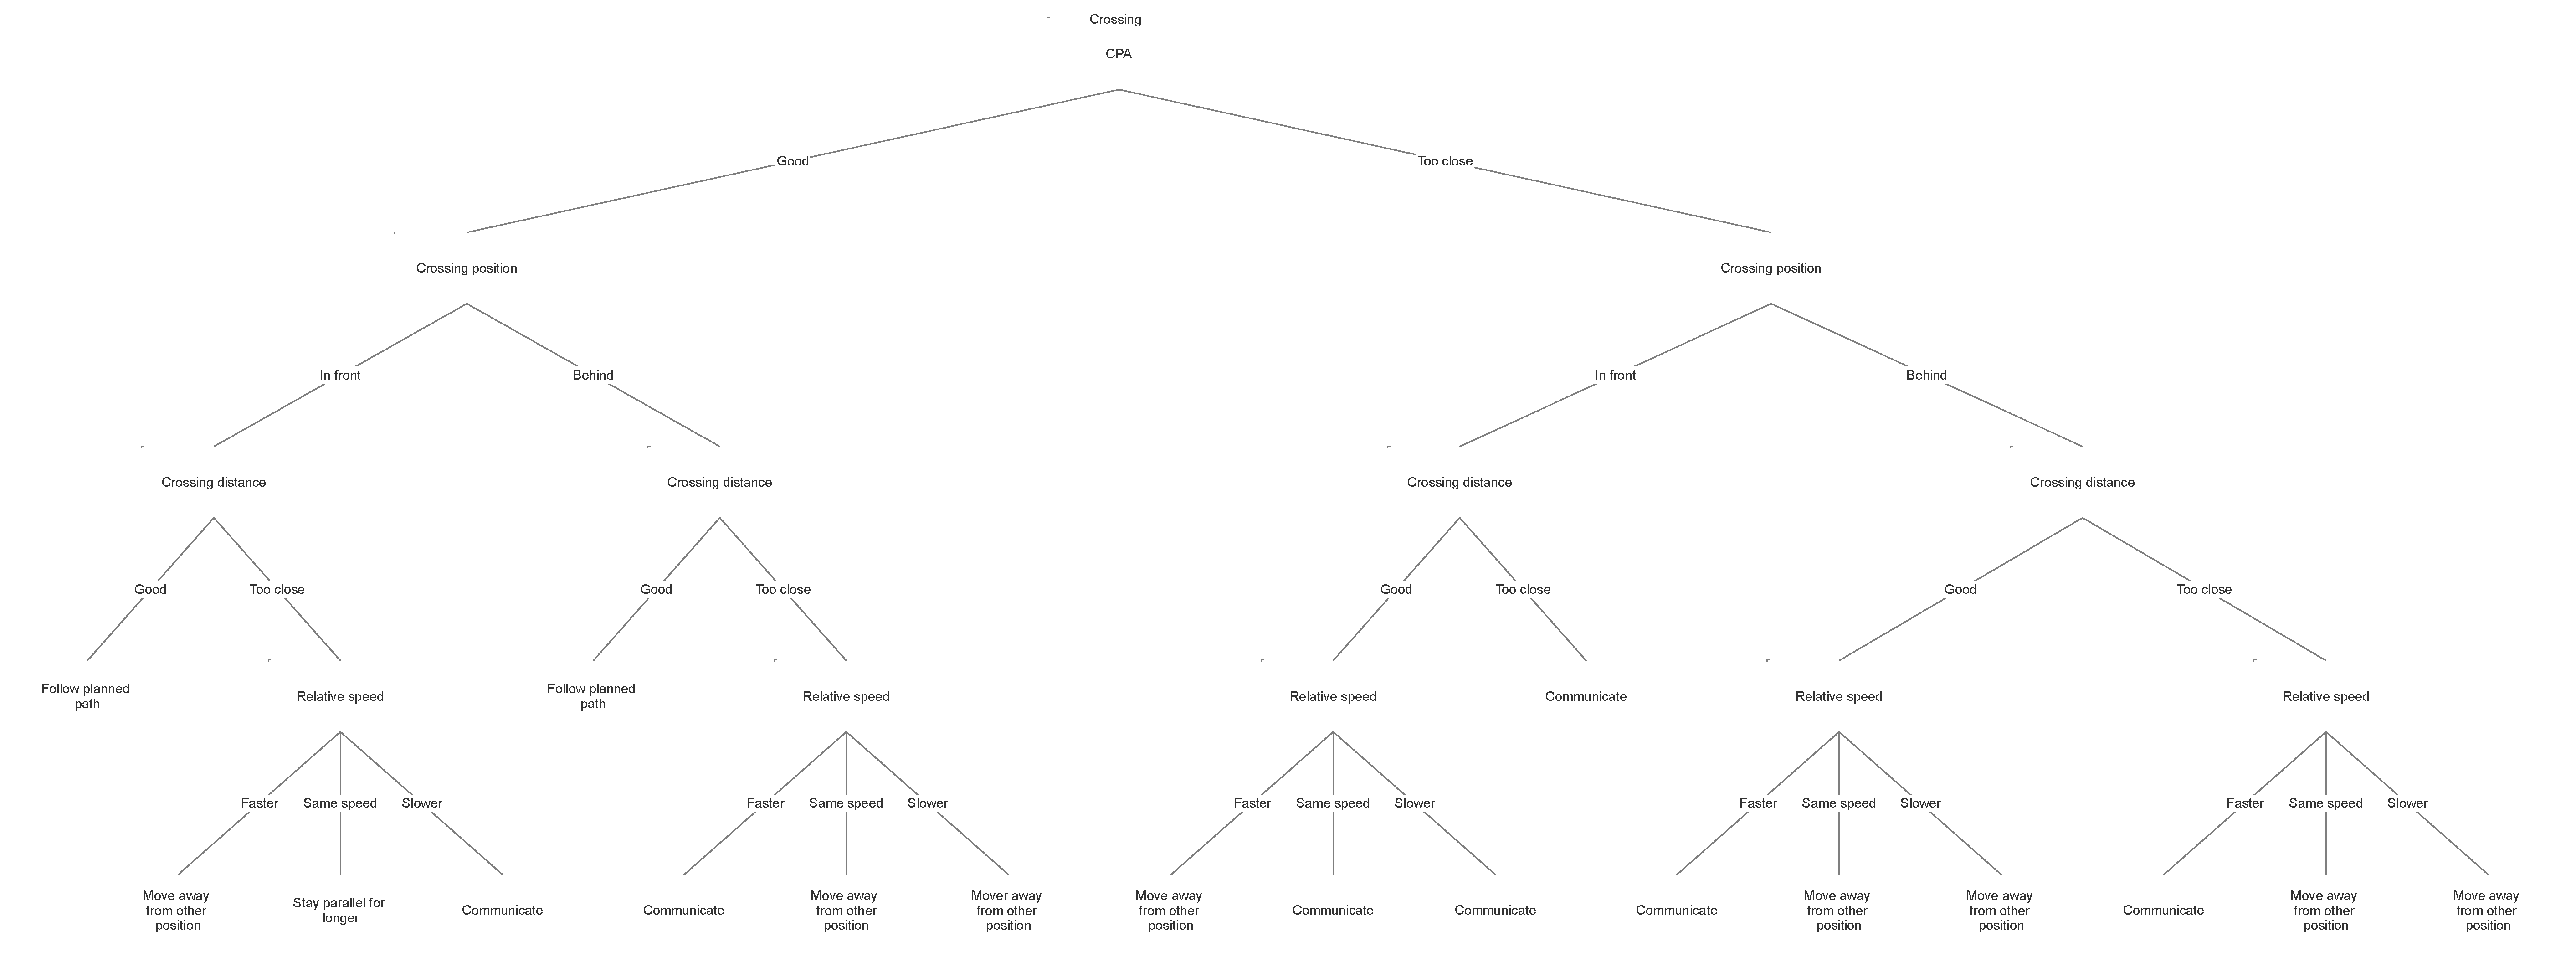
\includegraphics[width=.9\textheight, angle =90 ]{Crossing_decision_tree.png}
	\caption{Decision tree when crossing}
	\label{fig:Crossing_decision_tree}
\end{figure}


\begin{figure}[p]
	\centering
	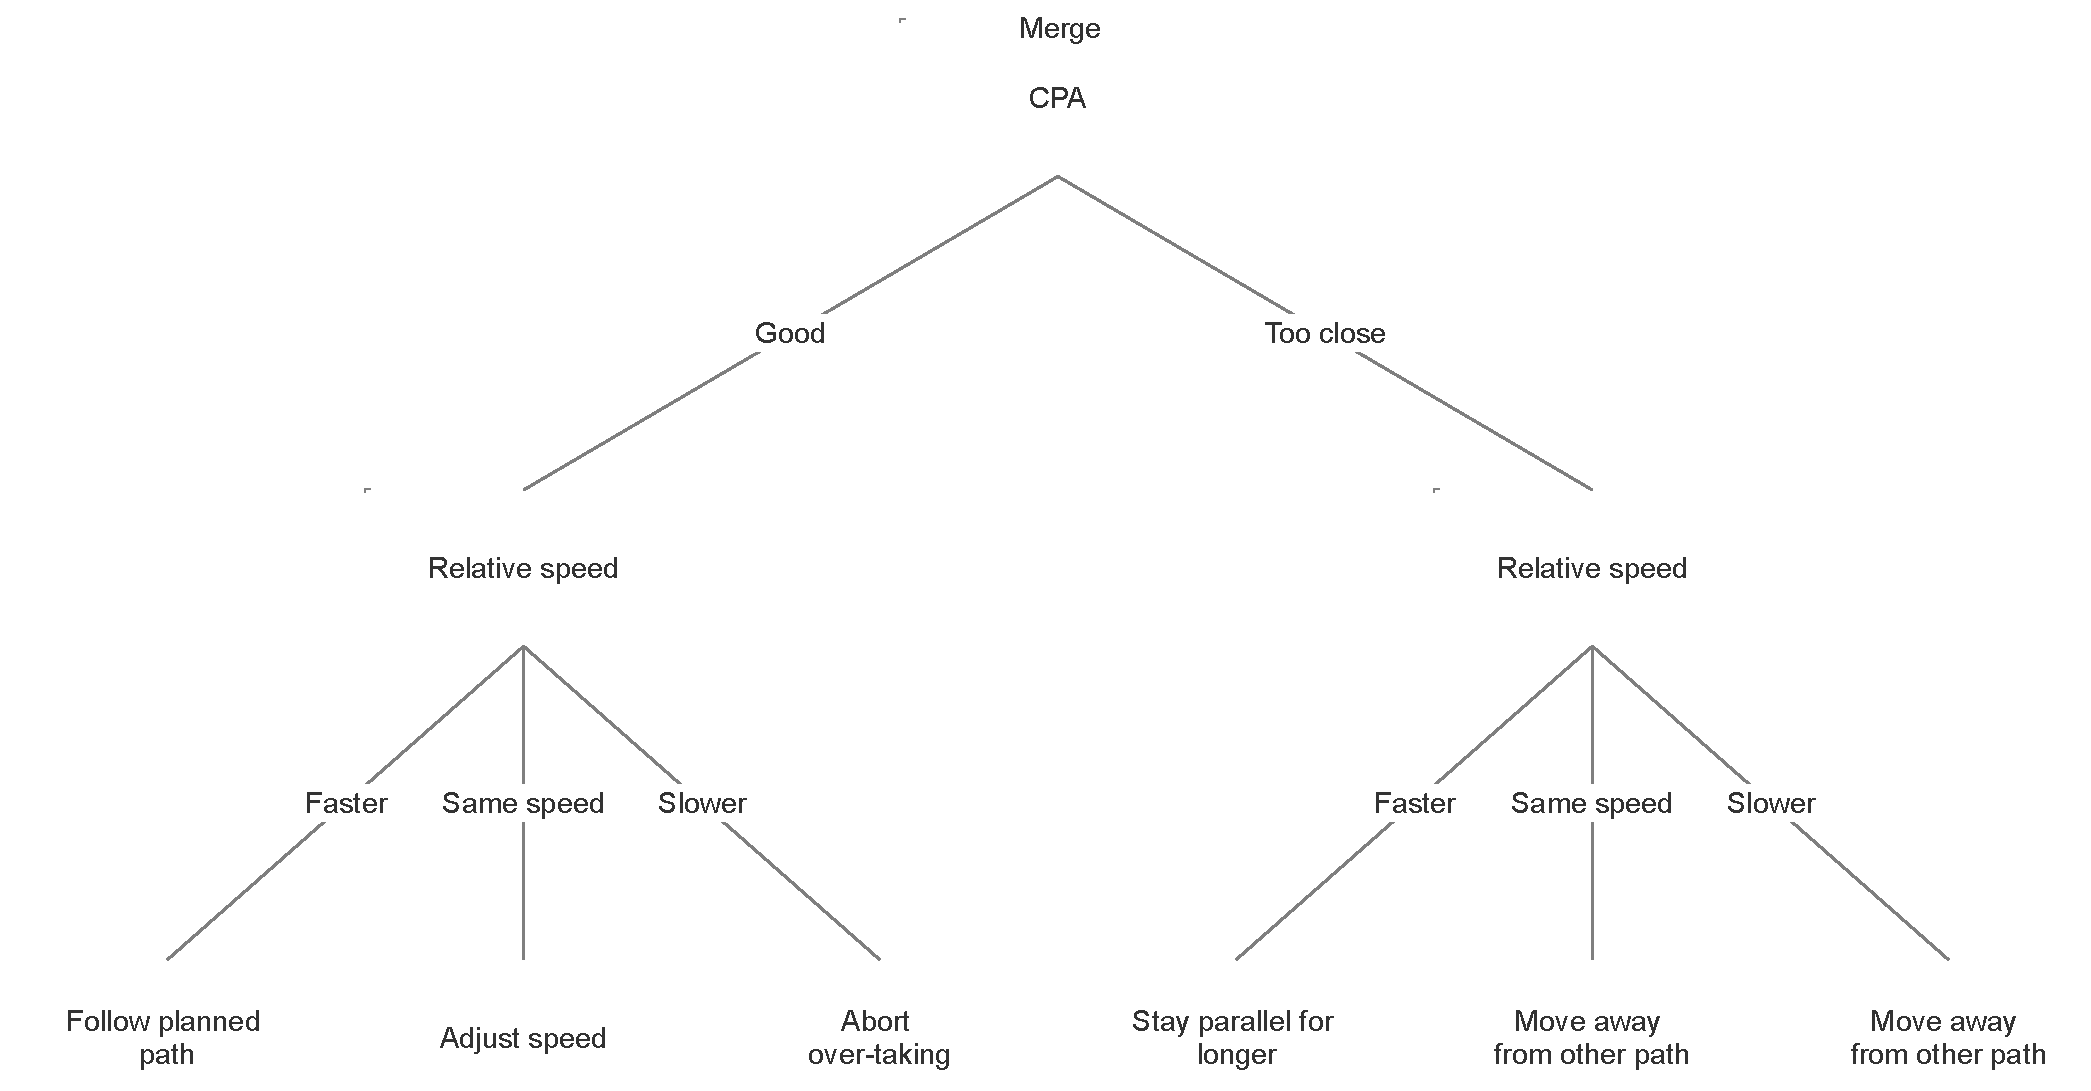
\includegraphics[width=.95\textwidth]{Merge_decision_tree.png}
	\caption{Decision tree when crossing}
	\label{fig:Merge_decision_tree}
\end{figure}


\begin{figure}[p]
	\centering
	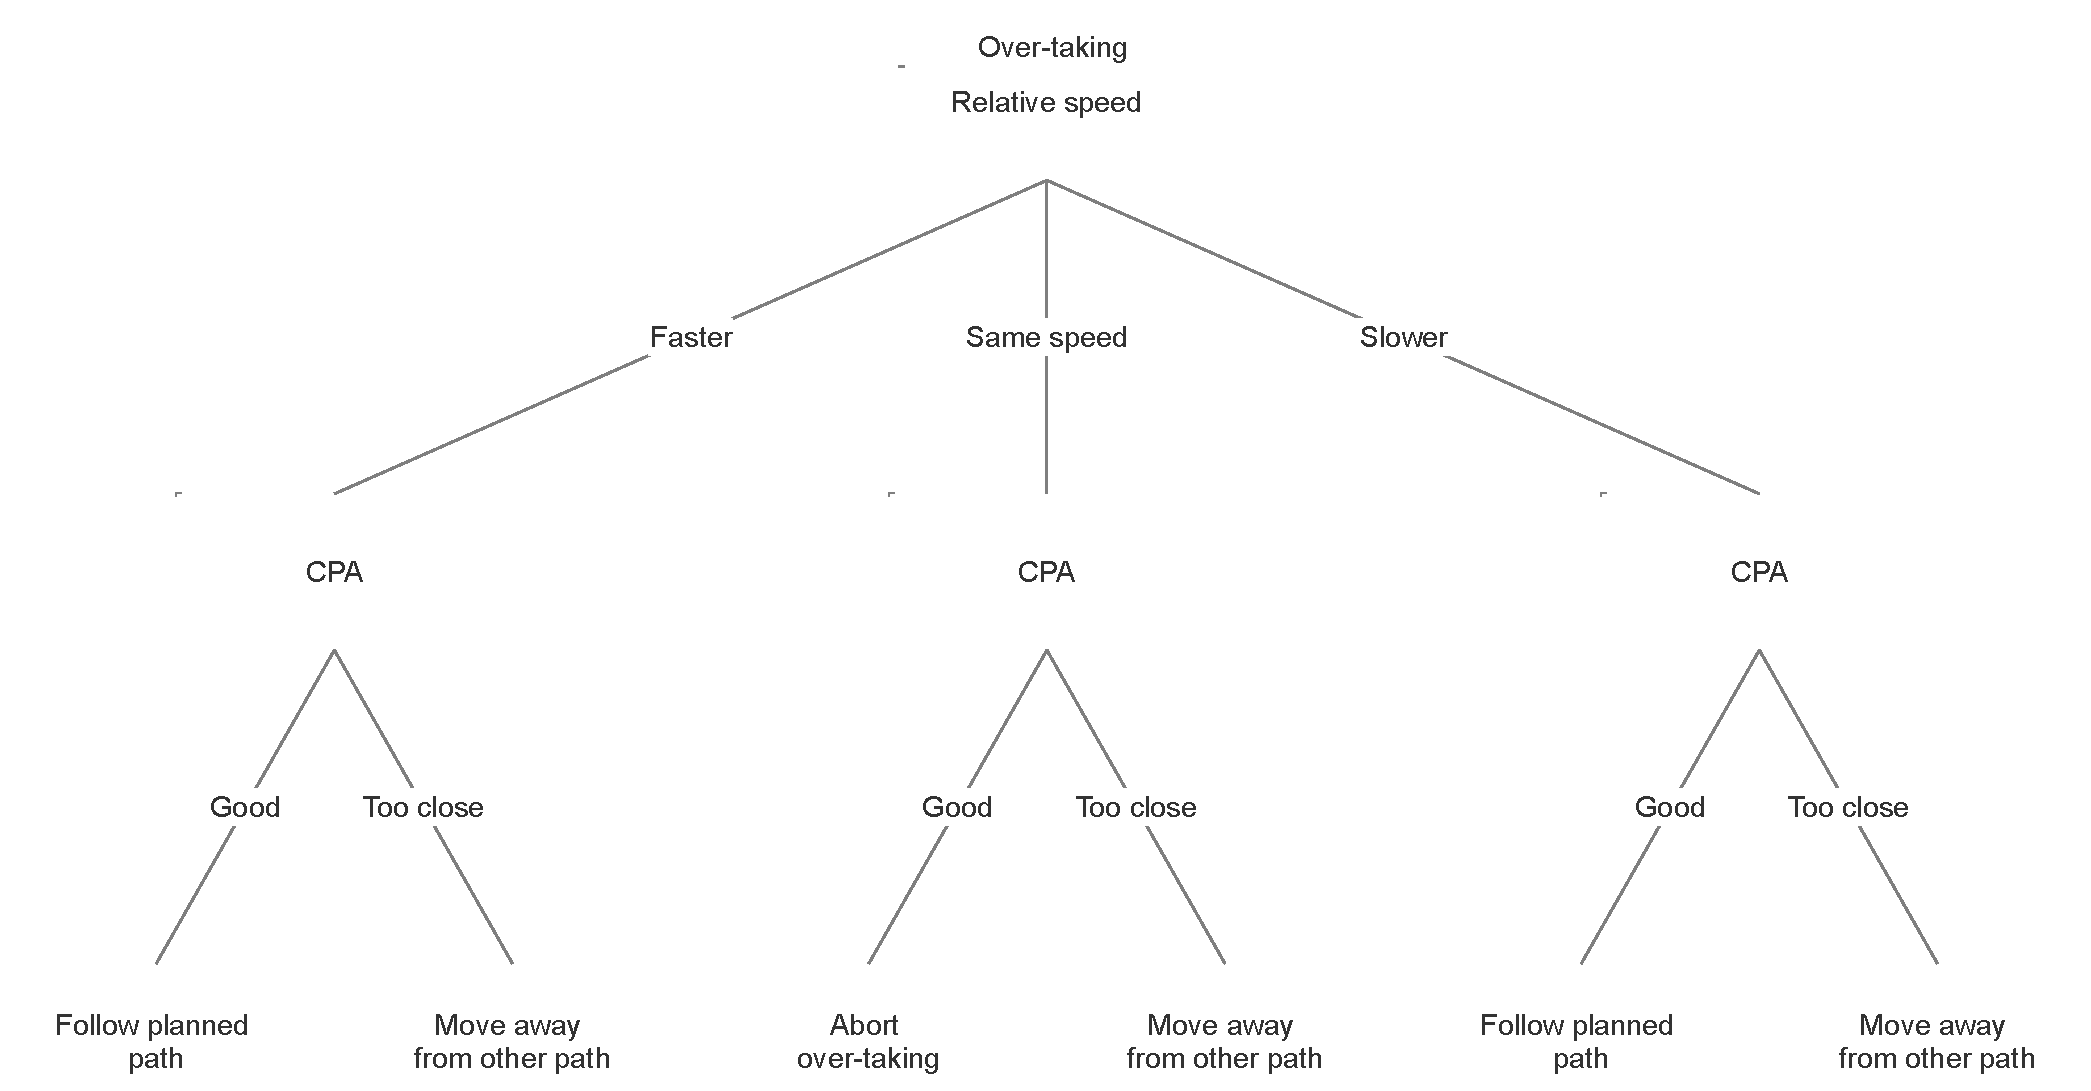
\includegraphics[width=.9\textwidth]{Over-taking_decision_tree.png}
	\caption{Decision tree when crossing}
	\label{fig:Over-taking_decision_tree}
\end{figure}


\begin{figure}[p]
	\centering
	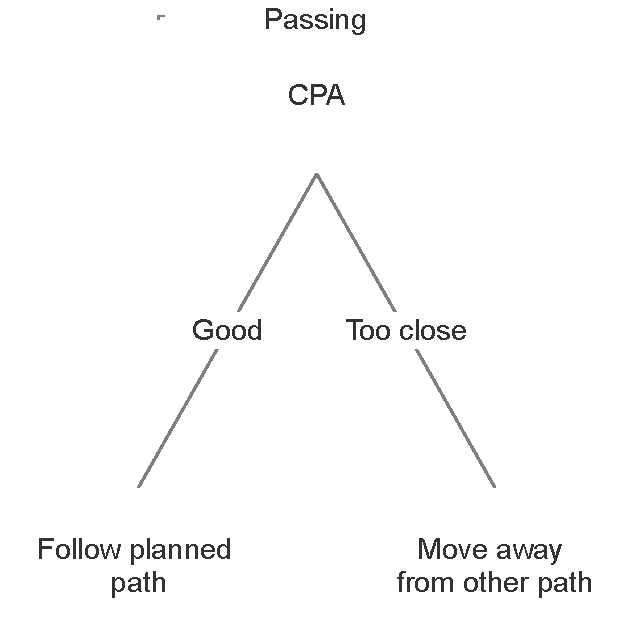
\includegraphics[width=0.2\textwidth]{Passing_decision_tree.png}
	\caption{Decision tree when crossing}
	\label{fig:Passing_decision_tree}
\end{figure}


